\chapter{Introduction to Dynamic Programming}

Dynamic programming (DP) is a method to solve complex problems by breaking them into smaller overlapping subproblems and building up solutions incrementally. It is essentially a technique for optimizing certain inefficient recursive algorithms by caching intermediate results for later reuse. 

\subsection{Key Concepts}
\begin{itemize}
    \item \textbf{Inefficiency in Recursion}: Many recursive algorithms are inefficient because they repeatedly solve the same subproblems.
    \item \textbf{Caching Results}: By storing intermediate results in a table (e.g., a hash table), we can avoid recalculating the same subproblem multiple times.
    \item \textbf{Efficiency}: This approach skips repeated recursive calls, speeding up the algorithm significantly.
\end{itemize}

\section{Elements of Dynamic Programming}

To effectively apply dynamic programming, the problem should have the following properties:

\begin{itemize}
    \item \textbf{Simple Subproblems}: The problem can be broken into smaller subproblems with the same structure.
    \item \textbf{Optimal Substructure}: The optimal solution of the overall problem depends on the optimal solutions of its subproblems.
    \item \textbf{Overlapping Subproblems}: Subproblems are solved multiple times during the computation.
\end{itemize}

\section{Case Study: Rod Cutting}
\begin{figure}[h!]
    \centering
    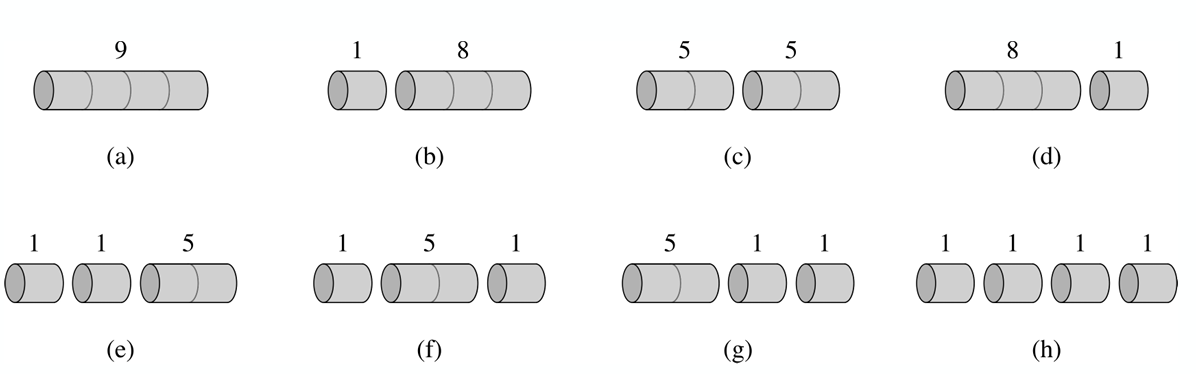
\includegraphics[width=1\linewidth]{immagini//capitolo 13/13_2.png}
    \caption{Enter Caption}
    \label{Example 1, here we show eight possible ways to cut a rod of lenght 4, the prices are shown on top}
\end{figure}
\subsection{Problem Statement}
Given a rod of length \(n\) inches and a table of prices \(p_i\) for rods of length \(i\), determine the maximum revenue obtainable by cutting the rod into smaller pieces and selling them.
\begin{figure}[h!]
    \centering
    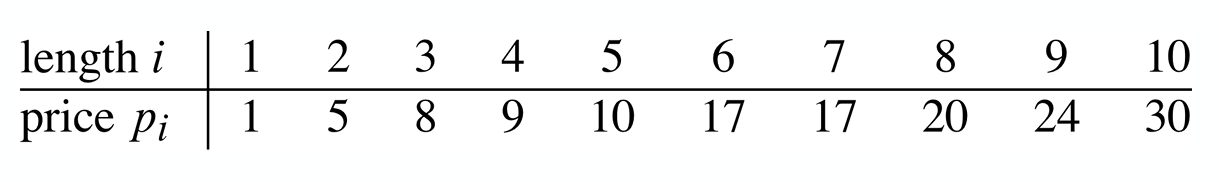
\includegraphics[width=1\linewidth]{immagini//capitolo 13/13_1.png}
    \caption{Another example of possible table of prices}
    \label{fig:enter-label}
\end{figure}
\textbf{Key Points:}
\begin{itemize}
    \item Rod cuts are integral lengths, and cutting incurs no cost.
    \item The solution involves finding the optimal way to cut the rod to maximize revenue.
\end{itemize}
The general formula for the maximum revenue \(r_n\) is:
\[
r_n = \max \big( p_n, r_1 + r_{n-1}, r_2 + r_{n-2}, \dots, r_{n-1} + r_1 \big) = \max_{1 \leq i \leq n} \big( p_i + r_{n-i} \big)
\]

\begin{itemize}
    \item \( p_n \): This represents the revenue obtained by selling the rod as is, without making any cuts. It is the simplest case.
    \item For the other \( n-1 \) arguments in the maximization formula, these correspond to the maximum revenue obtained by making an initial cut of the rod into two pieces of size \( i \) and \( n-i \), for each \( i = 1, 2, \dots, n-1 \).
    \item Once the rod is cut into two pieces, the revenues \( r_i \) and \( r_{n-i} \) are obtained by optimally cutting up those two pieces further.
    \item After making the first cut, the two resulting pieces can be treated as independent instances of the rod-cutting problem.
    \item The overall optimal solution incorporates the optimal solutions to these two related subproblems, maximizing the revenue from each of the two pieces. This ensures that the global solution is composed of optimal solutions to the subproblems.
\end{itemize}
In summary, the rod-cutting problem uses a divide-and-conquer strategy where the maximum revenue for a rod of length \( n \) is calculated by exploring all possible initial cuts, solving the subproblems for each resulting piece, and combining the results to achieve the maximum total revenue.

\subsection{Recursive Algorithm}

\begin{verbatim}
CUT-ROD(p, n):
    if n == 0:
        return 0  # No revenue is possible for a rod of length 0, so CUT-ROD return 0
    q = -infty
    for i = 1 to n:
        q = max(q, p[i] + CUT-ROD(p, n - i))  # Recursive call on the second piece
    return q
\end{verbatim}

\textbf{Explanation of the Code:}
\begin{itemize}
    \item \texttt{CUT-ROD} recursively computes the maximum revenue for a rod of length \(n\).
    \item The loop considers all possible first cuts (length \(i\)) and recursively solves for the remaining rod of length \(n-i\).
    \item It calls itself recursively many times with the same parameter values. 
    \item The result is the maximum revenue over all possible first cuts.
    \item This algorithm has an exponential running time \(T(n) = 2^n\), as it repeatedly solves the same subproblems.
\end{itemize}

\begin{figure}[h!]
    \centering
    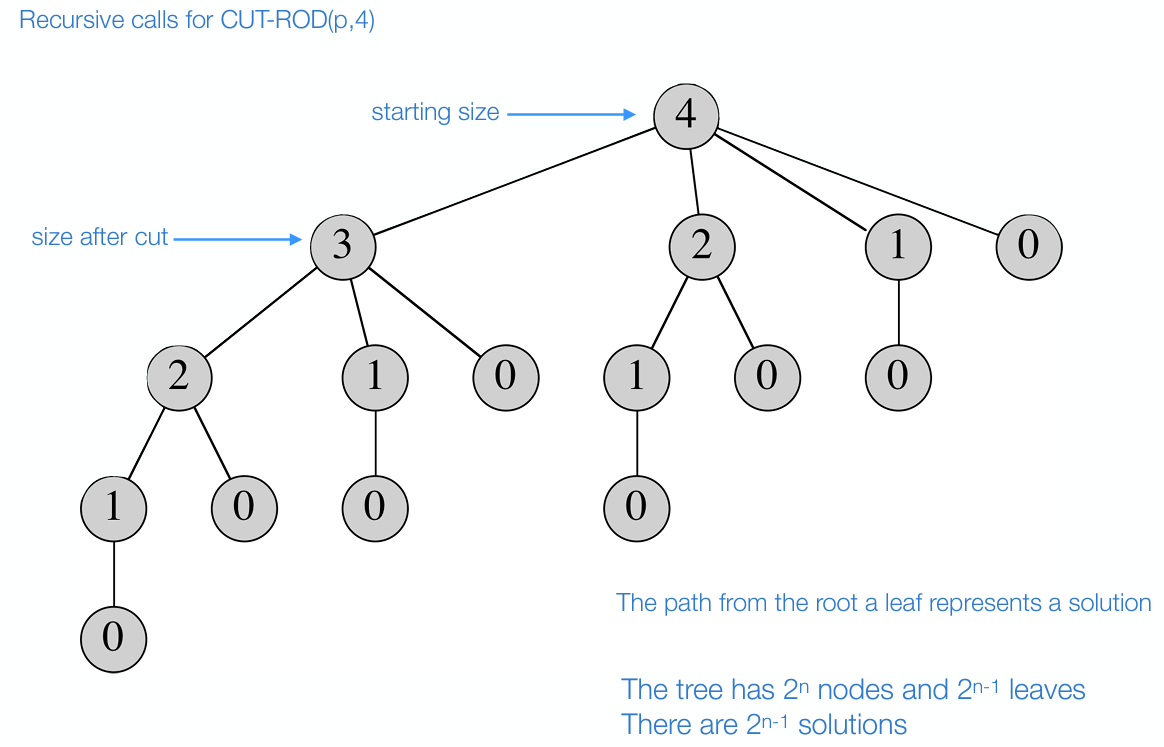
\includegraphics[width=1\linewidth]{immagini//capitolo 13/13_3.png}
    \label{CUT}
\end{figure}

\section{Improving Efficiency with Dynamic Programming}

\textbf{Key Idea:} Organize the algorithm to solve each subproblem only once, storing the solution in an appropriate data structure for reuse.

\begin{itemize}
    \item Use a data structure (e.g., array or hash table) to store solutions to subproblems.
    \item Retrieve stored solutions whenever a previously solved subproblem is encountered.
    \item Trade-off: Use more memory to store solutions but significantly reduce computation time.
\end{itemize}
\textbf{Performance:} Dynamic programming reduces the time complexity to polynomial when:
\begin{itemize}
    \item The input size is polynomial.
    \item The number of distinct subproblems is polynomial.
    \item Each subproblem can be solved in polynomial time.
\end{itemize}


\section{Memoization}

Memoization is a technique used in dynamic programming to store the solutions of subproblems to avoid redundant computations. There are two primary approaches to memoization. Both approaches have equivalent running times, but their implementations differ. Note that \textbf{memoization} is not the same as \textbf{memorization}.

\subsection{Top-Down Memoization}
In this approach, we solve the problem recursively in the usual way but store the solutions to subproblems as we compute them. This ensures that whenever we encounter a previously solved subproblem, we can simply retrieve the stored solution.

\subsection{Bottom-Up Memoization}
In this approach, we explicitly define the subproblems, order them by size in increasing order, and solve them iteratively. The solutions to smaller subproblems are used to solve larger ones. This approach avoids recursion and generally has lower constant factors compared to the top-down approach. This strategy usually has lower constant factors.



\section{Top-Down Memoization: Implementation}

\begin{verbatim}
MEMOIZED-CUT-ROD(p, n):
    let r[0, ..., n] be a new array
    for i = 0 to n:
        r[i] = -infinity
    return MEMOIZED-CUT-ROD-AUX(p, n, r)

MEMOIZED-CUT-ROD-AUX(p, n, r):
    if r[n] >= 0:  # Check for the stored solution
        return r[n]
    if n == 0:
        q = 0
    else:
        q = -infinity
        for i = 1 to n:
            q = max(q, p[i] + MEMOIZED-CUT-ROD-AUX(p, n - i, r))
    r[n] = q  # Store the solution for n
    return q
\end{verbatim}





\begin{figure}[h]
    \centering
    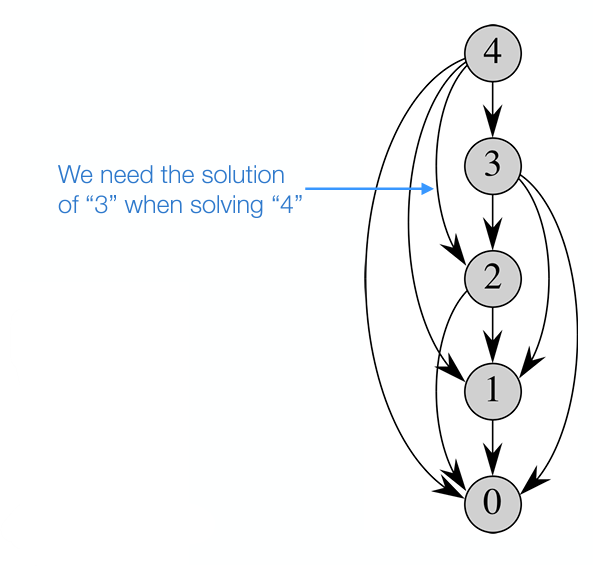
\includegraphics[width=0.75\linewidth]{immagini//capitolo 13/13_4.png}
    \caption{example of top-down memoization}
    \label{fig:enter-label}
\end{figure}

\textbf{Explanation of the Code:}
\begin{itemize}
    \item \texttt{MEMOIZED-CUT-ROD} initializes an array \texttt{r} to store solutions to subproblems.
    \item \texttt{MEMOIZED-CUT-ROD-AUX} performs the actual computation and checks if the solution for a given \(n\) is already stored. If so, it retrieves the solution; otherwise, it computes it recursively and stores it.
\end{itemize}
\newpage

\section{Bottom-Up Memoization: Implementation}

The bottom-up approach solves subproblems iteratively using their natural ordering. A subproblem of size \(i\) is solved before any subproblem of size \(j\) where \(i < j\).

\begin{verbatim}
BOTTOM-UP-CUT-ROD(p, n):
    let r[0, ..., n] be a new array
    r[0] = 0
    for j = 1 to n:
        q = -infinity
        for i = 1 to j:
            q = max(q, p[i] + r[j - i])  # Use the stored solution, no recursion
        r[j] = q
    return r[n]
\end{verbatim}

\textbf{Explanation of the Code:}
\begin{itemize}
    \item \texttt{BOTTOM-UP-CUT-ROD} initializes an array \texttt{r} to store solutions iteratively.
    \item Instead of recursive calls, the solution for \(r[j]\) is computed explicitly using stored solutions for smaller subproblems.
\end{itemize}
\textbf{Running Time:} The time complexity of both the top-down and bottom-up approaches is \(\Theta(n^2)\). Each subproblem is solved only once, and the time required is proportional to the number of subproblems.

\section{Printing the Optimal Solution}
To retrieve the cuts that produce the optimal solution, we extend the bottom-up approach to store the size of the first piece cut for each subproblem.

\begin{verbatim}
EXTEND-BOTTOM-UP-CUT-ROD(p, n):
    let r[0, ..., n] and s[1, ..., n] be new arrays
    r[0] = 0
    for j = 1 to n:
        q = -infinity
        for i = 1 to j:
            if q < p[i] + r[j - i]:
                q = p[i] + r[j - i]
                s[j] = i  # Store the optimal size i of the first piece to cut off 
                            when solving a subproblem of size j
        r[j] = q
    return r and s

PRINT-CUT-ROD-SOLUTION(p, n):
    (r, s) = EXTEND-BOTTOM-UP-CUT-ROD(p, n)
    while n > 0:
        print s[n]
        n = n - s[n]
\end{verbatim}

\textbf{Explanation of the Code:}
\begin{itemize}
    \item \texttt{EXTEND-BOTTOM-UP-CUT-ROD} calculates the maximum revenue \(r[j]\) and stores the size of the first cut \(s[j]\) for each subproblem.
    \item \texttt{PRINT-CUT-ROD-SOLUTION} reconstructs and prints the sequence of cuts leading to the optimal solution.
\end{itemize}

\begin{figure}[h!]
    \centering
    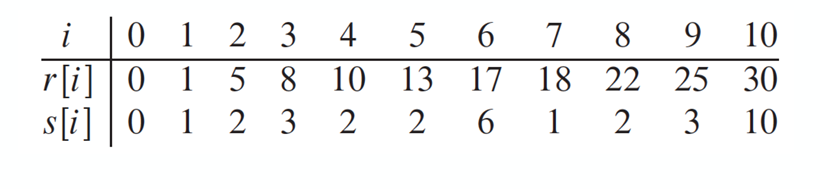
\includegraphics[width=1\linewidth]{immagini//capitolo 13/13_5.png}
    \caption{Result printed}
    \label{fig:enter-label}
\end{figure}

\section{Longest Common Subsequence (LCS)}

The Longest Common Subsequence (LCS) problem involves finding the longest subsequence that is common to two sequences \(x\) and \(y\), where a subsequence is a sequence derived from another sequence by deleting some elements without changing the order of the remaining elements.

\subsection{Problem Definition}
Given two sequences:
\begin{itemize}
    \item \(x = [a, b, c, b, d, a, b]\)
    \item \(y = [b, d, c, a, b, a]\)
\end{itemize}
Determine a longest common subsequence. For the example above, the LCS can be one of \(\{\text{bdab, bcab, bcba}\}\), each of length 4.

\subsection{Brute Force Algorithm}
A brute force approach checks every subsequence of \(x[1, \dots, m]\) to see if it is also a subsequence of \(y[1, \dots, n]\). \newline
\textbf{Analysis:}
\begin{itemize}
    \item Checking if a subsequence of \(x\) is a subsequence of \(y\) takes \(O(n)\), as it involves scanning \(y\).
    \item The number of subsequences of \(x\) is \(2^m\) because for each element I have two option: include it o don't include it.
    \item Therefore, the total cost is \(O(n \cdot 2^m)\).
\end{itemize}

\subsection{Simplification}
To simplify, we focus on the length of the LCS, \(c[x, y]\), which is unique. Using this, we can extend the algorithm to find one LCS. The strategy involves considering prefixes of \(x\) and \(y\), and expressing the length of their LCS in terms of smaller prefixes. \newline
\textbf{Definition:} \(c[i, j] = |\text{LCS}(x[1, \dots, i], y[1, \dots, j])|\)
\begin{itemize}
    \item \(c[i, j]\) is the length of the LCS for prefixes \(x[1, \dots, i]\) and \(y[1, \dots, j]\).
    \item Our goal is to compute \(c[m, n]\), the length of the LCS of \(x\) and \(y\). We want to express it in terms of other c[i,j] which we have previously calculate  $\forall i,j\in n,m$
\end{itemize}

\section{Proof of the Longest Common Subsequence (LCS) Algorithm}
\begin{align*}
    c[i, j] = \begin{cases}
        0, & \text{if } i = 0 \text{ or } j = 0, \\
        c[i-1, j-1] + 1, & \text{if } x[i] = y[j], \\
        \max\{c[i, j-1], c[i-1, j]\}, & \text{otherwise.}
    \end{cases}
\end{align*}

\subsection{Base Case}
\begin{itemize}
    \item \( c[i,j] = 0 \): This is true when one of the two sequences is empty because they have no elements in common.
\end{itemize}

\subsection{Case 1: \( x[i] = y[j] \)}
\begin{itemize}
    \item Assume there exists a common subsequence \( z[1,\dots,k] = \text{LCS}(x[1,\dots,i], y[1,\dots,j]) \) where \( c[i,j]=k \).
    \item Since \( x[i] = y[j] \), we can conclude that \( z[k] = x[i] = y[j] \). This is because if \( z \) does not include \( x[i] \) or \( y[j] \), then we could add this character to \( z \) to make it longer, contradicting the fact that \( z \) is the longest common subsequence (LCS).
    \item Hence, \( z[1,\dots,k-1] \) is a common subsequence (CS) of \( x[1,\dots,i-1] \) and \( y[1,\dots,j-1] \).
    \item \textbf{Claim}: \( z[1,\dots,k-1] \) is a \textit{longest} common subsequence (LCS) of \( x[1,\dots,i-1] \) and \( y[1,\dots,j-1] \).
\end{itemize}

\subsection{Proof of the Claim}
\begin{itemize}
    \item By contradiction, assume that \( w \) is a longer common subsequence than \( z \), such that \( |w| > k-1 \).
    \item Using a \textit{cut-and-paste argument}, concatenate \( w \) with \( z[k] \), forming \( w|z[k]| \).
    \item \( w|z[k]| \) is a common subsequence of \( x[1,\dots,i] \) and \( y[1,\dots,j] \) with a length greater than \( k \), which contradicts the assumption that \( z \) is the LCS.
    \item Therefore, \( c[i-1,j-1] = k-1 \), which implies \( c[i,j] = c[i-1,j-1] + 1 \).
\end{itemize}

\subsection{Case 2: \( x[i] \neq y[j] \)}
\begin{itemize}
    \item The proof for this case follows a similar reasoning and shows that:
    \[
    c[i,j] = \max(c[i-1,j], c[i,j-1])
    \]
\end{itemize}

\subsection{Optimal Substructure}
\begin{itemize}
    \item The problem exhibits \textit{optimal substructure}, meaning that the solution to the overall problem is composed of optimal solutions to its subproblems.
    \item If \( z = \text{LCS}(x, y) \), then any prefix of \( z \) is an LCS of a prefix of \( x \) and a prefix of \( y \).
\end{itemize}

\subsection{Recursive Algorithm}
\begin{verbatim}
LCS(x, y, i, j):
    # i, j are the last indices of x and y
    if i == 0 or j == 0:
        return 0  # Base case: one sequence is empty
    if x[i] == y[j]:
        return LCS(x, y, i-1, j-1) + 1  # Characters match
    else:
        return max(LCS(x, y, i-1, j), LCS(x, y, i, j-1))
\end{verbatim}

\textbf{Explanation of the Code:}
\begin{itemize}
    \item The function computes \(c[i, j]\) recursively based on the cases in the formula.
    \item Base cases handle when one sequence is empty.
    \item When \(x[i] = y[j]\), the LCS includes this character, and we compute the LCS for the remaining prefixes.
    \item When \(x[i] \neq y[j]\), the LCS is the maximum of excluding either \(x[i]\) or \(y[j]\).
\end{itemize}

\section{Worst Case Analysis for LCS}

The main computational challenge in the recursive LCS algorithm arises from the \texttt{else} clause, where two recursive calls are made. This creates an exponential growth in the number of subproblems solved. To illustrate, consider the case where $n=7$ and $m=6$. The recursion tree is as follows:

\begin{figure}[h!]
    \centering
    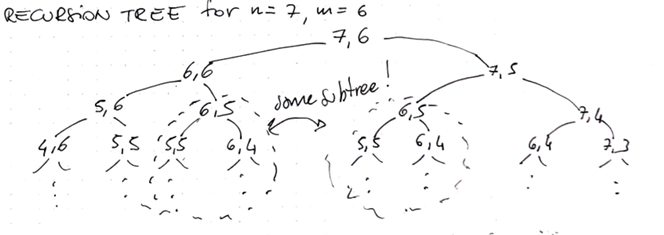
\includegraphics[width=1\linewidth]{immagini//capitolo 13/13_6.png}
    \label{fig:enter-label}
\end{figure}
As we observe, there are repeated subtrees, which indicate redundant computations. This redundancy can be eliminated using dynamic programming. The height of the recursion tree is $m+n$. Since it is a binary tree, each level introduces $2^i$ work, leading to a time complexity of $O(2^{m+n})$. However, LCS contains only $m \cdot n$ distinct subproblems. By storing the results of these subproblems, we avoid redundant computations. \newpage
The recurrence relation for the LCS problem is:
\[
T(n,m) = \begin{cases}
    T(n-1,m-1) + O(1), & \text{if } x[n] = y[m], \\
    T(n-1,m) + T(n,m-1) + O(1), & \text{otherwise}.
\end{cases}
\]
This exponential growth motivates the need for a bottom-up approach.

\subsection{Bottom-Up Memoized Algorithm}

The bottom-up approach systematically computes solutions for smaller subproblems first and uses them to construct the solution for larger subproblems. The pseudocode is as follows:

\begin{verbatim}
LCS-LENGTH(x, y, m, n)
    let b[1,...,m, 1,...,n] and c[0,...,m, 0,...,n] be new tables
    for i = 1 to m do
        c[i,0] = 0
    for j = 0 to n do
        c[0,j] = 0 #define the matrix c to zero
    for i = 1 to m do
        for j = 1 to n do
            if x[i] == y[j] then
                c[i,j] = c[i-1,j-1] + 1
                b[i,j] = " "  # northwest arrow
            else if c[i-1,j] >= c[i,j-1] then #if element up is >= than element left than
                c[i,j] = c[i-1,j] #copy from up
                b[i,j] = "↑"  # north arrow
            else
                c[i,j] = c[i,j-1] #copy from left
                b[i,j] = "←"  # west arrow
    return c, b
\end{verbatim}

\textbf{Explanation:}
\begin{itemize}
    \item The \texttt{c} table stores the lengths of LCS for prefixes of $x$ and $y$. b and c are matrixes.
    \item The \texttt{b} table stores arrows that indicate the direction of the optimal solution (northwest, north, or west).
    \item Base cases initialize the first row and column to 0, as an empty sequence has no common subsequence with any other sequence.
    \item This is a bottom up memoization algorithm because I start with the base case by setting the matrix element to 0 if i of j is equal to zero. In addition to that there isn't recursion.
\end{itemize}
\newpage
\subsection{Exercise}
Consider the sequences:
\begin{itemize}
    \item $x = A B C B D A B$
    \item $y = B D C A B A$
\end{itemize}

\begin{figure}[h!]
    \centering
    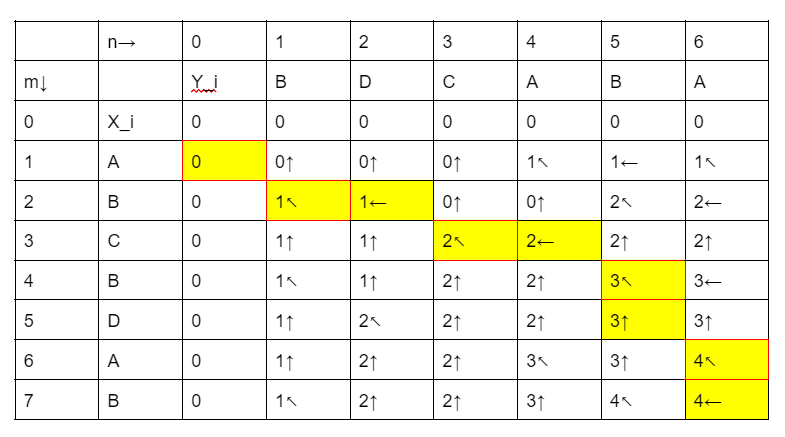
\includegraphics[width=1\linewidth]{immagini//capitolo 13/13_7.png}
    \label{fig:enter-label}
\end{figure}


\textbf{Instructions:}
\begin{itemize}
    \item If the characters at the current indexes match, copy the diagonal value and add 1.
    \item If they do not match, take the maximum value from the cell above or to the left. In case of a tie, prefer the top cell.
    \item Draw arrows in the \texttt{b} table to indicate the source of each value.
\end{itemize}

Starting from the bottom-right corner, trace back along the northwest arrows to construct the LCS and print a letter when you find the north-west arrow. Stop when a cell with value 0 is reached.

\subsection{Printing the LCS}

To print the LCS, we use the following recursive function:

\begin{verbatim}
PRINT-LCS(b, x, i, j)
    if i == 0 or j == 0
        return
    if b[i,j] == "↖ " then # north-west arrow 
        PRINT-LCS(b, x, i-1, j-1)
        print x[i]
    else if b[i,j] == "↑" then
        PRINT-LCS(b, x, i-1, j)  # Go up
    else
        PRINT-LCS(b, x, i, j-1)  # Go left
\end{verbatim}

\textbf{Explanation:}
\begin{itemize}
    \item The function recursively traverses the \texttt{b} table.
    \item It prints characters of $x$ only when a northwest arrow is encountered starting from bottom left.
    \item This ensures the correct order of characters in the LCS.
\end{itemize}

\section{Dynamic Programming: Text Justification}

\subsection{Problem Statement}
Given a sequence of words and a limit on the number of characters per line (\textit{line width}), we aim to insert line breaks in the sequence such that the lines are printed neatly.
\begin{figure}[h!]
    \centering
    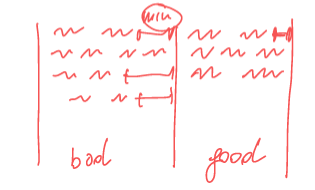
\includegraphics[width=0.75\linewidth]{immagini//capitolo 13/13_8.png}
    \label{fig:enter-label}
\end{figure}
\paragraph{Input:} An array of words $l = w[0, \ldots, n-1]$, where $|l| = n$.

\paragraph{Scoring Rule:} 
Suppose we consider the words from index $i$ to $j$ ($w[i], w[i+1], \ldots, w[j]$). We define the \textbf{badness} of this justification as:
\[
\text{badness}(i, j) =
\begin{cases}
+\infty & \text{if } j+1-i > \text{page\_width}, \\
\big(\text{page\_width} - (len(w[i]+ w[i+1]+\ldots+w[j] + 1)\big)^2 & \text{otherwise.}
\end{cases}
\]
Our goal is to divide the words in order to minimize the total badness.

\subsection{Brute-Force Algorithm}
A naive algorithm examines all possible ways to divide the sequence into lines. This approach has a complexity of $\mathcal{O}(2^n)$, which is impractical for large inputs.

\subsection{Dynamic Programming Approach}
We can reduce the complexity by leveraging the structure of the problem.

\paragraph{Subproblems:} 
Define the cost $c[i]$ as the minimum badness of dividing the suffix $w[i, \ldots, n-1]$ into lines:
\[
c[i] = \min\big(\text{badness}(i, j) + c[j+1]\big) \quad \text{for all } j \in [i, n-1].
\]
Here:
\begin{itemize}
    \item Computing $\text{badness}(i, j)$ requires $\mathcal{O}(1)$ operations.
    \item The recurrence considers up to $n-i+1$ choices for $j$, so each $c[i]$ computation is $\mathcal{O}(n)$.
\end{itemize}
Thus, the overall complexity is $\mathcal{O}(n^2)$.

\subsection{Example}
Suppose we have the following \textbf{Words:} ``diamonds are girl's best friends'' and a
\textbf{Page Width} equal to 12.

\paragraph{Word Table:}
\[
\begin{array}{|c|c|c|}
\hline
i & \text{Word} & \text{Length} \\
\hline
0 & \text{diamonds} & 8 \\
1 & \text{are} & 3 \\
2 & \text{girls} & 5 \\
3 & \text{best} & 4 \\
4 & \text{friends} & 7 \\
\hline
\end{array}
\]

\paragraph{Greedy Approach:}
In this approach, we fill each line as much as possible before moving to the next line. The resulting layout and badness are as follows:

\[
\begin{array}{|c|c|}
\hline
\text{Line} & \text{Badness} \\
\hline
\text{diamonds are} & 0 \\
\text{girls best} & 2^2 \\
\text{friends} & 5^2 \\
\hline
\text{Total Badness} & 29 \\
\hline
\end{array}
\]

\paragraph{Dynamic Programming Approach:}
The dynamic programming solution minimizes the total badness. The resulting layout and badness are as follows:

\[
\begin{array}{|c|c|}
\hline
\text{Line} & \text{Badness} \\
\hline
\text{diamonds} & 4^2 \\
\text{are girls} & 3^2 \\
\text{best friends} & 0 \\
\hline
\text{Total Badness} & 25 \\
\hline
\end{array}
\]
In the DP approach, we compute the badness of all possible divisions and store intermediate results to avoid recomputation. This results in a more optimal layout than the greedy approach.

\subsection{Optimal Solution}
To find the best way to justify the text, we calculate the \textbf{badness matrix}, which stores the cost of fitting words from index $i$ to $j$ on one line. The process involves two main steps:
\begin{enumerate}
    \item Compute the badness for each possible grouping of words.
    \item Use dynamic programming to find the minimum cost and reconstruct the optimal solution.
\end{enumerate}

\paragraph{Badness Matrix Table:}
\[
\begin{array}{|c|c|c|c|c|c|}
\hline
i \downarrow \backslash j \rightarrow & 0 \, (\text{diamonds}) & 1 \, (\text{are}) & 2 \, (\text{girls}) & 3 \, (\text{best}) & 4 \, (\text{friends}) \\
\hline
0 & 16 & 0 & \infty & \infty & \infty \\
1 & - & 81 & 9 & \infty & \infty \\
2 & - & - & 49 & 4 & \infty \\
3 & - & - & - & 64 & 0 \\
4 & - & - & - & - & 25 \\
\hline
\end{array}
\]
The matrix is half-empty because it represents only valid groupings of words.

\paragraph{Dynamic Programming Arrays:}
We define two arrays:
\begin{itemize}
    \item \textbf{minCost:} Stores the minimum cost for justifying the suffix starting at word $i$.
    \item \textbf{index:} Stores the index used to reconstruct the optimal solution.
\end{itemize}

\subsection{Step-by-Step Computation}
\begin{figure}[h!]
    \centering
    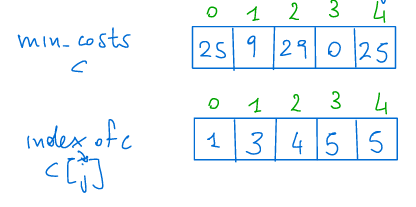
\includegraphics[width=1\linewidth]{immagini//capitolo 13/13_9.png}
    \label{fig:enter-label}
\end{figure}


\begin{itemize}
    \item \textbf{First Iteration:} By default we start from the last word (\textit{friends}), we set the last element of minCost with the value of the badness(n-1,n-1) e index[n-1] = n, where n is the number of words. Therefore $minCost[4] = 25$ and $index[4] = 5$. 
    \item \textbf{Second Iteration:} From now on, we compute for each $i$ from $n-2$ to 0 the quantity $\text{badness}(i,j) + \text{minCost}[j+1]$ for all $j \in (i, n-1)$ and select the minimum. This will be $\text{minCost}[i]$, and we set $\text{index}[i] = j+1$ where $j$ is the index used to obtain $\text{minCost}[i]$. In our calculations, we may encounter cases where we compute $\text{minCost}[j^*]$ where $j^* > n-1$; in this case, set $\text{minCost}[j^*] = 0$. \newline
    Now i = n-2=3 and j$\in (3,4)$. We compute:
    \begin{align*}
         &\text{badness}(3,3) + minCost[4] = 64 + 25 = 89 \\
         &\text{badness}(3,4) + minCost[5] = 0 + 0   = 0
    \end{align*}
    We set minCost[3] = 0 and index[3] = 5. 
    \item \textbf{Third Iteration:} Now i = 2 and j$\in (2,3,4)$. We compute:
    \begin{align*}
        &\text{badness}(2,2) + minCost[3] = 49 + 0 = 49 \\
        &\text{badness}(2,3) + minCost[4] = 4 + 25 = 29 \\
        &\text{badness}(2,4) + minCost[5] = \infty + 0 = \infty
    \end{align*}
    We set minCost[2] = 29 and index[2] = 4. 
    \item \textbf{Fourth Iteration:} Now i = 1 and j$\in (1,2,3,4)$. We compute:
    \begin{align*}
        &\text{badness}(1,1) + minCost[2] = 81 + 29 = 110 \\
        &\text{badness}(1,2) + minCost[3] = 9 + 0 = 9 \\
        &\text{badness}(1,3) + minCost[4] = \infty + 25= \infty \\
        &\text{badness}(1,4) + minCost[5] = \infty + 0 = \infty
    \end{align*}
    We set minCost[1] = 9 and index[1] = 3. 
    \item \textbf{Fifth Iteration:} Now i = 0 and j$\in (0,1,2,3,4)$. We compute:
    \begin{align*}
        &\text{badness}(0,0) + minCost[1] = 16 + 9 = 25 \\
        &\text{badness}(0,1) + minCost[2] = 0 + 29 = 29 \\
        &\text{badness}(0,2) + minCost[3] = \infty + 0 = \infty \\
        &\text{badness}(0,3) + minCost[4] = \infty + 25= \infty \\
        &\text{badness}(0,4) + minCost[5] = \infty + 0 = \infty
    \end{align*}
    We set minCost[0] = 25 and index[0] = 1.
\end{itemize}

\paragraph{Optimal Layout:}
To print the words, we look at the first element of the $\text{index}$ vector. This indicates the index up to which we can print the words. For example, if the element $\text{index}[0]$ is 1, it means that we can print the words up to word 1 excluded, therefore only word 0, which is "diamond", and then go to a new line. To understand how many words to place on the second line, we use the element that was in the previously examined position, i.e., 1, as the index of the vector. $\text{index}[1] = 3$, so we can print words 1 and 2, which are "are girls". We apply this procedure again and obtain that in the third line we can put the words up to number $\text{index}[3] = 5$, therefore words 3 and 4. If we had had other words, we could have continued.
\paragraph{Optimal Justification:}
\begin{verbatim}
diamonds
are girls
best friends
\end{verbatim}

\subsection{Pseudocode}
\textbf{Main Algorithm:}
\begin{verbatim}
TEXT-JUSTIFICATION(W, page_width)
input: an array of words W and page_width
output: minimum Cost and list of indexes for optimal justification

// Initialize the badness matrix
let badness[0 .. len(W)-1, 0 .. len(W)-1] be empty
for i <- 0 to len(W)-1 do
    badness[i,i] <- page_width - len(W[i])
    for j <- i+1 to len(W)-1 do
        badness[i,j] <- badness[i,j-1] - len(W[j]) - 1

// Compute badness values
for i <- 0 to len(W)-1 do
    for j <- i to len(W)-1 do
        if badness[i,j] < 0 then
            badness[i,j] <- infinity
        else:
            badness[i,j] <- badness[i,j]^2

// Calculate minCost and index arrays
let minCost[0 .. len(W)-1], index[0 .. len(W)-1] be empty
for i <- len(W)-1 to 0 do
    minCost[i] <- badness[i, len(W)-1]
    index[i] <- len(W)-1
    for j <- len(W)-1 to i+1 do
        if badness[i,j-1] != infinity and minCost[i] > badness[i,j-1] + minCost[j] then
            minCost[i] <- badness[i,j-1] + minCost[j]
            index[i] <- j
return (minCost, index)
\end{verbatim}

\textbf{Text Printing Algorithm:}
\begin{verbatim}
PRINT-JUSTIFIED-TEXT(W, page_width)
(minCost, index) <- TEXT-JUSTIFICATION(W, page_width)
i <- 0
do:
    j <- index[i]
    for k <- i to j-1 do:
        if k != j-1 then
            print(W[k] + " ") // Add space for all but last word
        else:
            print(W[k]) // Print last word in the line
    print("\n") // Move to the next line
    i <- j
while i < len(W)
\end{verbatim}

\section{All Pairs Shortest Path Problem}
The \textbf{All Pairs Shortest Path (APSP)} problem involves finding the shortest path between every pair of vertices in a graph \( G = (V, E) \). 

The \textbf{Floyd-Warshall Algorithm} solves the APSP problem in \( \Theta(V^3) \) time, which is efficient for dense graphs. This algorithm:
\begin{itemize}
    \item Works with directed graphs with weighted edges.
    \item Handles negative weights but requires that there are no negative weight cycles.
    \item Considers intermediate vertices in paths.
\end{itemize}

\subsection{Intermediate Vertices and Paths}
To compute the shortest path, the algorithm considers intermediate vertices in a path. Let:
\[
p = \langle v_1, v_2, \dots, v_l \rangle
\]
represent a path, where intermediate vertices are:
\[
\{v_2, v_3, \dots, v_{l-1}\}.
\]

\subsection{Key Lemma}
\textbf{Lemma 1:}  
Given a weighted directed graph \( G = (V, E) \) with \( w: E \to \mathcal{R} \), let:
\[
p = \langle v_0, v_1, \dots, v_k \rangle
\]
be the \textbf{Shortest Path (SP)} from \( v_0 \) to \( v_k \). For any \( i, j \) such that \( 0 \leq i \leq j \leq k \), the subpath:
\[
p_{ij} = \langle v_i, v_{i+1}, \dots, v_j \rangle
\]
is the shortest path from \( v_i \) to \( v_j \).

\textbf{Proof:}  
If a shorter path \( p'_{ij} \) exists, \( p \) would no longer be the shortest path. Thus, \( p_{ij} \) must also be the shortest path.

\subsection{Intermediate Nodes in Shortest Paths}

Given \( V = \{v_1, v_2, \dots, v_n\} \), consider a subset \( \{v_1, v_2, \dots, v_k\} \) for some \( k < n \). For any \( i, j \in V \), consider all paths from \( i \) to \( j \) whose intermediate vertices are drawn from \( \{v_1, \dots, v_k\} \), and let \( p \) be the shortest path (SP) among them.

Now consider the subset \( \{v_1, v_2, \dots, v_{k-1}\} \):
\begin{itemize}
    \item If \( k \) is \textbf{not an intermediate node of \( p \)}, then all intermediate nodes of \( p \) are in \( \{v_1, v_2, \dots, v_{k-1}\} \). In this case, the SP from \( i \) to \( j \) with intermediates in \( \{v_1, v_2, \dots, v_{k-1}\} \) is also the SP with intermediates in \( \{v_1, v_2, \dots, v_k\} \).

    \item If \( k \) \textbf{is an intermediate node of \( p \)}, then the path can be expressed as \( p = i \to k \to j \). Here, \( p_1 = i \to k \) and \( p_2 = k \to j \) are subpaths of \( p \). By Lemma 1, \( p_1 \) is the SP from \( i \) to \( k \) with intermediates in \( \{v_1, \dots, v_k\} \), and \( p_2 \) is the SP from \( k \) to \( j \) with intermediates in \( \{v_1, \dots, v_k\} \).
\end{itemize}

This observation leads directly to the recurrence relation that will be used to compute the shortest paths incrementally as we consider more intermediate nodes.

\subsection{Recursive Solution}
Let \( d^{(k)}_{ij} \) represent the weight of the shortest path from \( i \) to \( j \) using only the vertices \( \{v_1, v_2, \dots, v_k\} \) as intermediate vertices.

\paragraph{Base Case (\( k = 0 \)):}
\[
d^{(0)}_{ij} = 
\begin{cases} 
w(i, j), & \text{if } (i, j) \in E, \\
0, & \text{if } i = j, \\
\infty, & \text{otherwise.}
\end{cases}
\]

\paragraph{Recursive Step (\( k \geq 1 \)):}
\[
d^{(k)}_{ij} = 
\min\big(d^{(k-1)}_{ij}, d^{(k-1)}_{iK} + d^{(k-1)}_{Kj}\big).
\]

Here:
\begin{itemize}
    \item \( d^{(k-1)}_{ij} \): The shortest path without using vertex \( k \) as an intermediate.
    \item \( d^{(k-1)}_{iK} + d^{(k-1)}_{Kj} \): The path through vertex \( k \).
\end{itemize}

\paragraph{Final Answer:}  
The matrix \( D^{(n)} \) gives \( d^{(n)}_{ij} = \delta(i, j) \) for all \( i, j \in V \).

\subsection{Algorithm Description}
The input is a weight matrix \( W \) where:
\[
w_{ij} = 
\begin{cases} 
0, & \text{if } i = j, \\
w(i, j), & \text{if } (i, j) \in E, \\
\infty, & \text{otherwise.}
\end{cases}
\]
The output is a matrix \( D^{(n)} \) containing shortest path distances. \newline
\textbf{Pseudocode:}
\begin{verbatim}
FLOYD-WARSHALL(W)
    n = rows[W]
    D^(0) <- W
    for k = 1 to n do
        for i = 1 to n do
            for j = 1 to n do
                D^(k)[i][j] = min(D^(k-1)[i][j], 
                                  D^(k-1)[i][k] + D^(k-1)[k][j])
    return D^(n)
\end{verbatim}

\paragraph{Explanation:}
\begin{itemize}
    \item \( D^{(0)} \): Initialize using the weight matrix \( W \).
    \item For each intermediate vertex \( k \), update the distance matrix \( D \) by considering paths through \( k \).
    \item The algorithm iterates over all \( i, j \) pairs for each \( k \), resulting in a cubic complexity \( \Theta(V^3) \).
\end{itemize}

\subsection{Complexity Analysis}
The Floyd-Warshall Algorithm has a time complexity of:
\[\Theta(V^3)\] which is efficient for dense graphs. It computes the shortest paths for all vertex pairs in \( V \), making it a versatile algorithm for graph analysis.

\section{Purpose of the \( \Pi \)-Matrix in Floyd-Warshall Algorithm}

The \( \Pi \)-matrix (or predecessor matrix) is used in the Floyd-Warshall algorithm to reconstruct the shortest paths between all pairs of vertices. While the \( D \)-matrix stores the minimum distances, the \( \Pi \)-matrix tracks the predecessors in the shortest paths.

\subsection{Role of the \( \Pi \)-Matrix}
\begin{itemize}
    \item \textbf{Path Reconstruction:}
    The entry \( \Pi[i][j] \) represents the vertex immediately before \( j \) in the shortest path from \( i \) to \( j \). By following the predecessor chain in the \( \Pi \)-matrix, it is possible to reconstruct the shortest path.

    \item \textbf{Initialization:}
    \begin{itemize}
        \item If there is an edge from \( i \) to \( j \), \( \Pi[i][j] \) is initialized to \( i \) because \( i \) is the predecessor of \( j \).
        \item If there is no direct edge between \( i \) and \( j \), \( \Pi[i][j] \) is initialized to \( \text{None} \) or \( -1 \) to indicate that no path exists initially.
    \end{itemize}

    \item \textbf{Update Rule:}
    During the algorithm's execution, whenever a shorter path from \( i \) to \( j \) through \( k \) is found, \( \Pi[i][j] \) is updated to reflect the new predecessor:
    \[
    \Pi[i][j] = \Pi[k][j]
    \]
\end{itemize}

\subsection{Example of Use}
Suppose the following \( \Pi \)-matrix is obtained after running the Floyd-Warshall algorithm:
\[
\Pi = 
\begin{bmatrix}
- & 1 & 1 & 2 \\
2 & - & 2 & 2 \\
3 & 3 & - & 3 \\
4 & 4 & 4 & -
\end{bmatrix}
\]

To find the shortest path from vertex \( 1 \) to \( 4 \):
\begin{enumerate}
    \item Start at vertex \( 4 \) (the destination).
    \item Look at \( \Pi[1][4] = 2 \), which means the predecessor of \( 4 \) in the shortest path is \( 2 \).
    \item Now look at \( \Pi[1][2] = 1 \), which means the predecessor of \( 2 \) in the shortest path is \( 1 \).
    \item Thus, the shortest path is \( 1 \to 2 \to 4 \).
\end{enumerate}

\subsection{Benefits}
The \( \Pi \)-matrix provides the following advantages:
\begin{itemize}
    \item It complements the \( D \)-matrix: while \( D \) gives the shortest distances, \( \Pi \) enables the reconstruction of the actual paths.
    \item It avoids recomputing the path dynamically by storing the predecessor information during the algorithm execution.
\end{itemize}

\subsection{Summary}
The \( \Pi \)-matrix ensures that the Floyd-Warshall algorithm not only computes the shortest distances but also provides a way to determine the actual sequence of vertices in each shortest path. This is particularly useful in applications requiring explicit paths, such as navigation systems or route planning.


\section{Floyd-Warshall Algorithm: Example and Solution}

\subsection{Problem Description}
We are given a directed weighted graph \( G = (V, E) \) with the following edges and weights:
\begin{itemize}
    \item \( 1 \to 2 \): Weight = 3
    \item \( 1 \to 5 \): Weight = -4
    \item \( 2 \to 3 \): Weight = 4
    \item \( 2 \to 5 \): Weight = 7
    \item \( 3 \to 4 \): Weight = -5
    \item \( 4 \to 2 \): Weight = 1
    \item \( 5 \to 4 \): Weight = 6
\end{itemize}
The goal is to compute the shortest paths between all pairs of vertices using the Floyd-Warshall algorithm.

\subsection{Graph Representation}
The graph can be represented as follows:

\subsection{Algorithm Description}
The Floyd-Warshall algorithm computes the shortest path between all pairs of vertices by iteratively considering intermediate vertices. The key recurrence relation is:
\[
d^{(k)}_{ij} = \min\big(d^{(k-1)}_{ij}, d^{(k-1)}_{iK} + d^{(k-1)}_{Kj}\big),
\]
where \( d^{(k)}_{ij} \) represents the shortest path from vertex \( i \) to vertex \( j \), considering the first \( k \) vertices as potential intermediates.

\subsection{Initialization}
The initial distance matrix \( D^{(0)} \) and predecessor matrix \( \Pi^{(0)} \) are defined as follows:

\subsection{Conclusion}
After all iterations, the final \( D^{(n)} \) matrix contains the shortest path distances between all pairs of vertices, and the \( \Pi^{(n)} \) matrix contains the predecessors for reconstructing the paths.
\begin{figure}[h!]
    \centering
    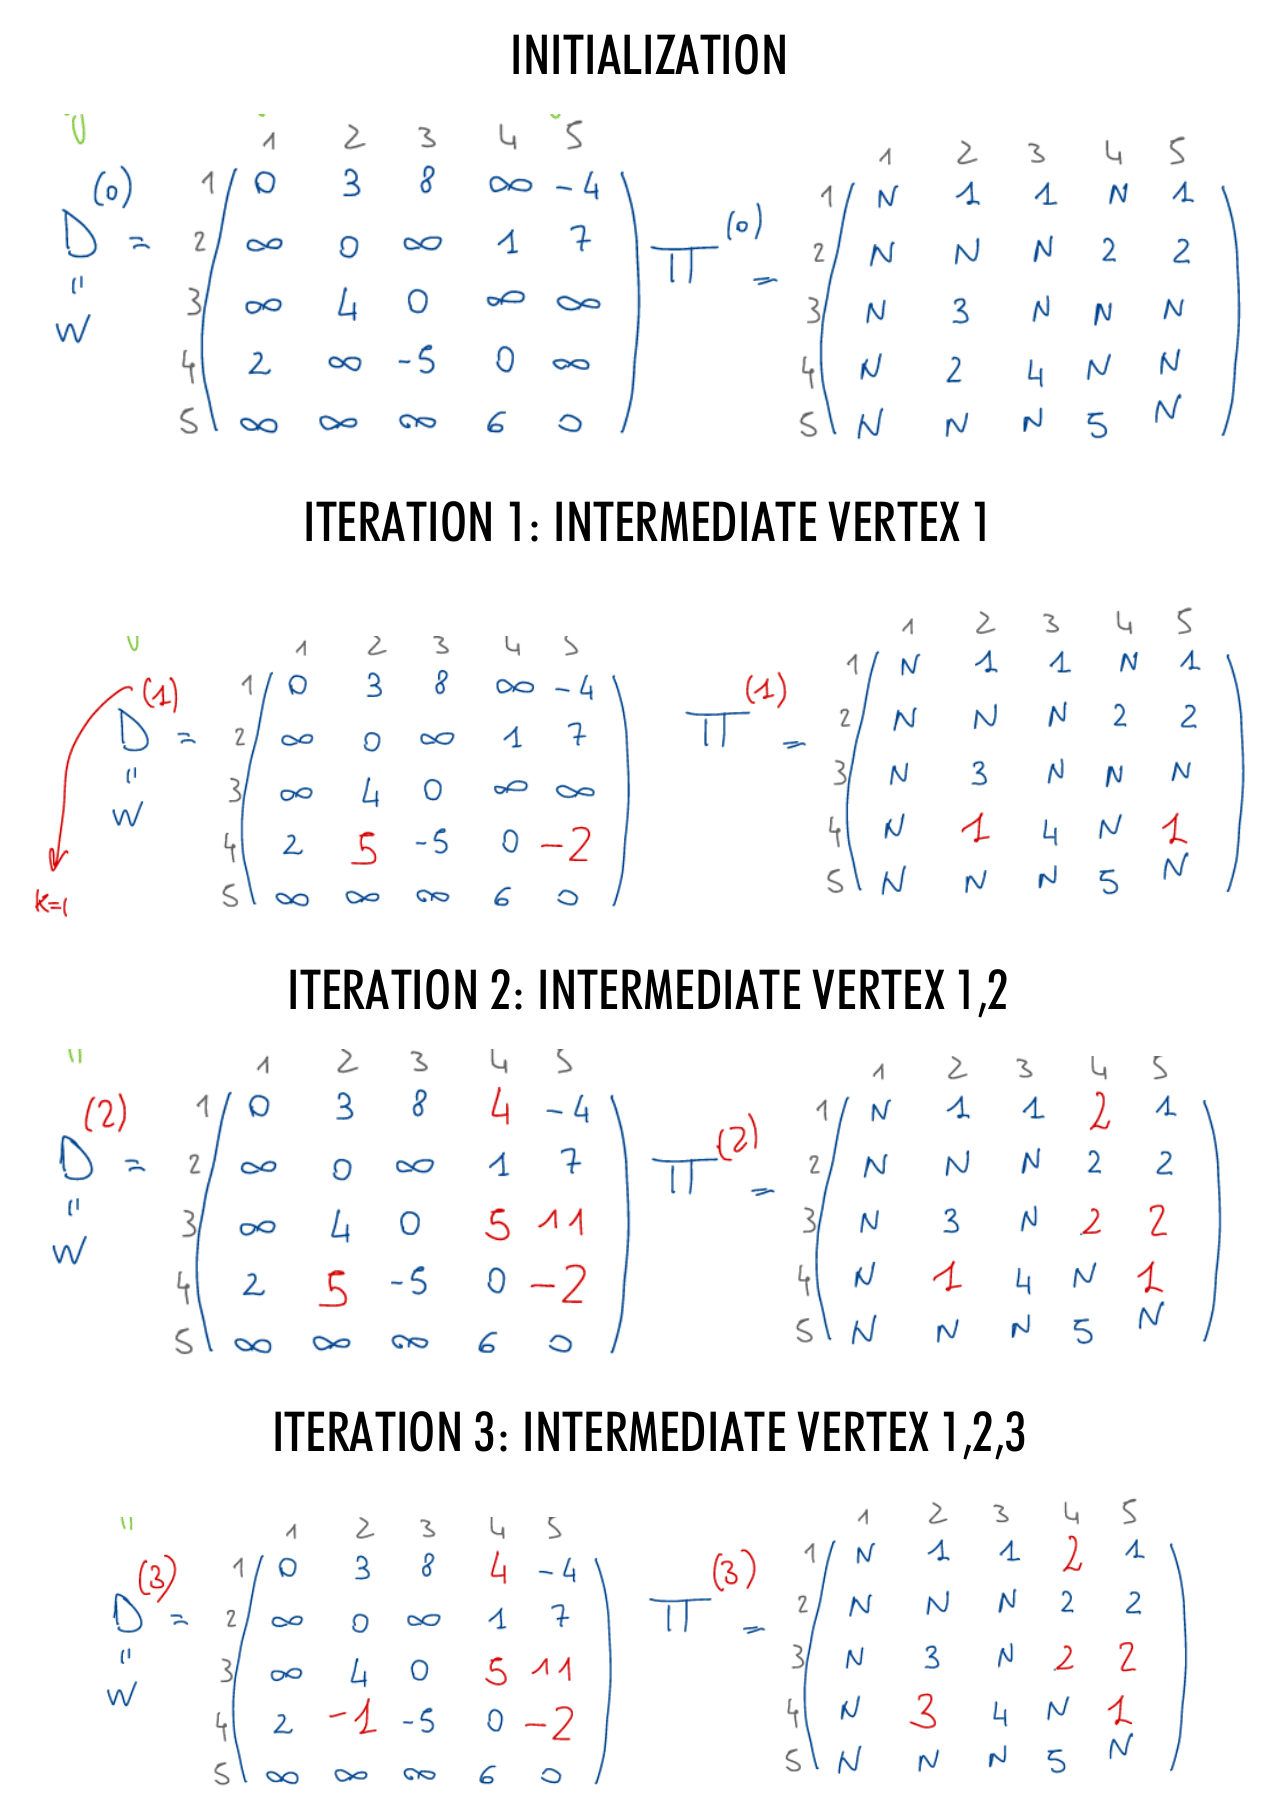
\includegraphics[width=0.7\linewidth]{immagini//capitolo 14 esercizio/INITIALIZATION-1.png}
    \caption{Enter Caption}
    \label{fig:enter-label}
\end{figure}

\newpage
\begin{figure}[h!]
    \centering
    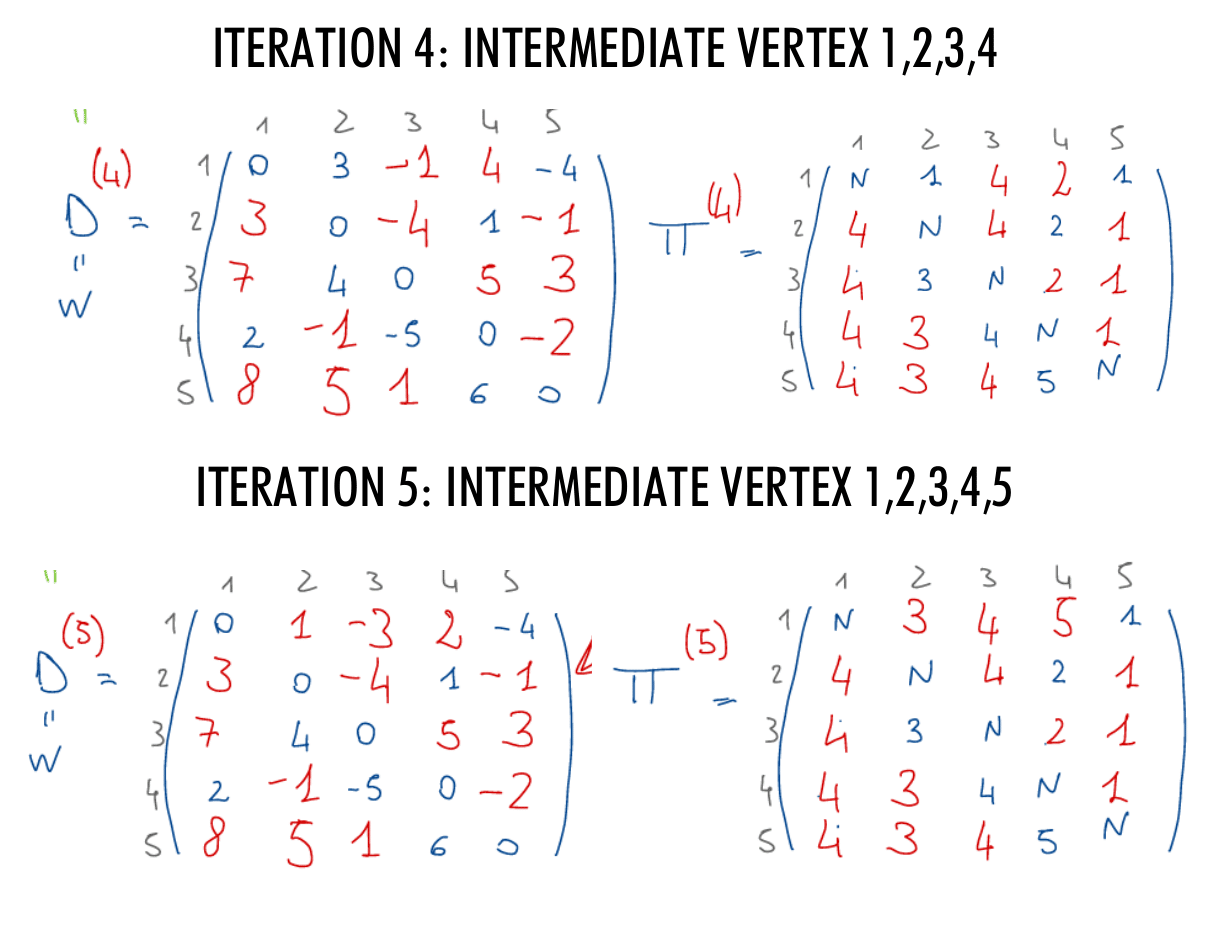
\includegraphics[width=0.75\linewidth]{immagini//capitolo 14 esercizio/INITIALIZATION-2.png}
    \caption{Enter Caption}
    \label{fig:enter-label}
\end{figure}

\begin{figure}[h!]
    \centering
    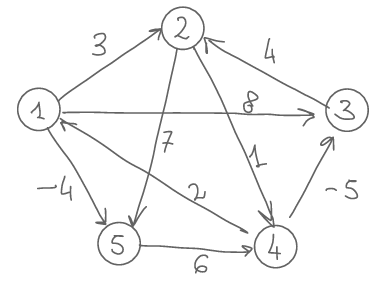
\includegraphics[width=0.75\linewidth]{immagini//capitolo 14 esercizio/14_grafo.png}
\end{figure}


